
\documentclass[12pt,a4paper]{report}
\usepackage[utf8]{inputenc}
\usepackage[T1]{fontenc}
\usepackage{graphicx}
\usepackage{geometry}
\usepackage{listings}
\usepackage{xcolor}
\usepackage{bookmark}
\usepackage{hyperref}
\usepackage{colortbl}
\usepackage{booktabs}
\usepackage{array}
\usepackage{parskip}
\usepackage{titlesec}
\usepackage{enumitem}
\usepackage{tikz}
\usepackage{float}

% ---- Page geometry ----
\geometry{a4paper, top=2.2cm, bottom=2.2cm, left=2.5cm, right=2.5cm}

% ---- Hyperref ----
\hypersetup{colorlinks=false, hidelinks}

% ---- Section formatting ----
\titleformat{\chapter}[hang]{\large\bfseries}{}{0pt}{}[\vspace{-4pt}\rule{\textwidth}{0.6pt}]
\titlespacing*{\chapter}{0pt}{0pt}{8pt}
\titleformat{\section}{\normalsize\bfseries}{\thesection}{1em}{}
\titlespacing*{\section}{0pt}{8pt}{4pt}

% ---- Colors ----
\definecolor{codegreen}{rgb}{0,0.6,0}
\definecolor{codegray}{rgb}{0.5,0.5,0.5}
\definecolor{codepurple}{rgb}{0.58,0,0.82}
\definecolor{backcolour}{rgb}{0.95,0.95,0.92}
\definecolor{tableheader}{rgb}{0.18,0.38,0.60}
\definecolor{tablealt}{rgb}{0.93,0.96,1.0}

% ---- Code style ----
\lstdefinestyle{mystyle}{
    backgroundcolor=\color{backcolour},
    commentstyle=\color{codegreen},
    keywordstyle=\color{magenta},
    numberstyle=\tiny\color{codegray},
    stringstyle=\color{codepurple},
    basicstyle=\ttfamily\scriptsize,
    breakatwhitespace=false,
    breaklines=true,
    captionpos=b,
    keepspaces=true,
    numbers=left,
    numbersep=5pt,
    showspaces=false,
    showstringspaces=false,
    showtabs=false,
    tabsize=2,
    frame=single,
    rulecolor=\color{codegray}
}
\lstset{style=mystyle}

% ---- New column type for tables ----
\newcolumntype{L}[1]{>{\raggedright\arraybackslash}p{#1}}
\newcolumntype{C}[1]{>{\centering\arraybackslash}p{#1}}

% ============================================================
\begin{document}
% ============================================================

% ============================
% PAGE 1 — COVER PAGE
% ============================
\begin{titlepage}
    \centering
    \IfFileExists{lpulogo.png}{
\includegraphics[width=0.38\textwidth]{lpulogo.png}}{\vspace*{1.5cm}}

    \vspace{0.5cm}
    \LARGE\textbf{Lovely Professional University}\\[0.3cm]
    \large Department of Computer Applications\\[0.2cm]
    \large\textbf{CAP777 — CA2: Project 1}\\[1.8cm]

    {\Huge\textbf{EduBridge}}\\[0.3cm]
    {\large\textit{An Online Teacher--Student Booking Platform}}\\[2.0cm]

    \begin{minipage}{0.48\textwidth}
        \begin{flushleft}\large
            \emph{Submitted By:}\\[4pt]
            \textbf{Nitish Kumar}\\
            Roll No: \textbf{RD2526B60}\\
            Reg No: \textbf{12515641}
        \end{flushleft}
    \end{minipage}
    \hfill
    \begin{minipage}{0.48\textwidth}
        \begin{flushright}\large
            \emph{Submitted To:}\\[4pt]
            \textbf{Simranpreet Kaur}\\
            Faculty, CA Dept.
        \end{flushright}
    \end{minipage}

    \vfill
    \large\textbf{2nd Semester Project Report}\\
    \large\textbf{April 2026}
\end{titlepage}

% ============================
% PAGE 2 — DECLARATION
% ============================
\newpage
\thispagestyle{plain}
{\large\bfseries Declaration}\\[0.6pt]
\rule{\textwidth}{0.6pt}

\vspace{1cm}
I, \textbf{Nitish Kumar} (Registration Number: \textbf{12515641}), hereby declare that the project report entitled \textbf{``EduBridge: An Online Teacher--Student Booking Platform''}, submitted for the partial fulfillment of \textbf{CAP777 (CA2: Project 1)}, is my own original work.

\vspace{0.4cm}
No part of this project has been submitted elsewhere for any other examination. All referenced sources have been duly acknowledged.

\vspace{3cm}
\noindent\textbf{Name:} Nitish Kumar\\[0.5cm]
\textbf{Registration No.:} 12515641\\[0.5cm]
\textbf{Date:} April 2026\\[0.5cm]
\textbf{Signature:} \underline{\hspace{5cm}}

% ============================
% PAGE 3 — ABSTRACT
% ============================
\newpage
\thispagestyle{plain}
{\large\bfseries Abstract}\\[0.6pt]
\rule{\textwidth}{0.6pt}

\vspace{0.6cm}
\textbf{EduBridge} is a web-based educational platform that connects students with verified teachers for online tutoring sessions. The system provides three role-specific portals — Student, Teacher, and Administrator — each with dedicated features for booking, communication, and management.

\vspace{0.4cm}
Students can search for teachers by subject or language, view profiles and ratings, book sessions, and communicate through a built-in messaging system. Teachers manage their availability, session schedules, and earnings. Administrators oversee platform activity, handle verifications, and monitor analytics.

\vspace{0.4cm}
The platform is built using \textbf{Core PHP} with a \textbf{MySQL} database accessed through \textbf{PDO}, a responsive front-end using \textbf{Bootstrap 5.3} and \textbf{JavaScript}, all served via \textbf{Apache (XAMPP)}. The project demonstrates a complete, functional web application following structured MVC principles, with clean UI, secure data handling, and role-based access control.

% ============================
% PAGE 4 — INTRODUCTION + PROBLEM STATEMENT
% ============================
\newpage
\thispagestyle{plain}
{\large\bfseries Introduction \& Problem Statement}\\[0.6pt]
\rule{\textwidth}{0.6pt}

\vspace{0.4cm}
\textbf{Introduction}

\vspace{0.2cm}
EduBridge is a multi-portal web application that simplifies the process of finding and booking quality teachers online. The platform caters to students seeking personalised academic assistance and to experienced educators who want to offer tutoring services digitally. The Admin portal ensures platform integrity through manual verification and monitoring.

\vspace{0.5cm}
\textbf{Problem Statement}

\vspace{0.2cm}
Finding a reliable and qualified tutor involves several friction points:

\begin{itemize}[leftmargin=1.5em, itemsep=2pt]
    \item No centralised, trustworthy platform to discover and verify teachers.
    \item Booking sessions manually via calls or WhatsApp is inefficient and untracked.
    \item Payments and session tracking are managed informally with no digital record.
    \item Students have no structured way to review teachers or track their learning history.
    \item Teachers lack a professional space to manage their schedule, income, and reputation.
    \item Administrators have no streamlined tools to verify educators or moderate disputes.
\end{itemize}

\vspace{0.4cm}
EduBridge addresses these gaps by providing an end-to-end, role-aware digital ecosystem for structured online tutoring.

% ============================
% PAGE 5 — OBJECTIVES + SCOPE
% ============================
\newpage
\thispagestyle{plain}
{\large\bfseries Objectives \& Project Scope}\\[0.6pt]
\rule{\textwidth}{0.6pt}

\vspace{0.4cm}
\textbf{Objectives}

\begin{itemize}[leftmargin=1.5em, itemsep=3pt]
    \item Build a multi-role web platform for students, teachers, and administrators.
    \item Allow students to search, filter, and book verified teachers online.
    \item Provide teachers with scheduling, session management, and earnings dashboards.
    \item Implement secure role-based login, registration, and profile management.
    \item Enable an in-app messaging system for student--teacher communication.
    \item Give admins tools to verify teachers, manage reports, and view analytics.
    \item Deliver a fully responsive, professional UI using Bootstrap 5.3.
    \item Ensure data security using PDO prepared statements and input validation.
    \item Generate a structured booking flow: search → profile → slot → payment → session.
\end{itemize}

\vspace{0.5cm}
\textbf{Project Scope}

\begin{itemize}[leftmargin=1.5em, itemsep=3pt]
    \item \textbf{Included:} User registration, login, OTP verification, 3 role portals, teacher search and discovery, time-slot booking, messaging system, reviews and ratings, admin dashboard, teacher verification workflow, responsive landing page.
    \item \textbf{Not Included:} Native mobile app, video conferencing integration, payment gateway (placeholders only), email automation.
    \item \textbf{Target Users:} School/college students seeking tutoring and experienced teachers willing to teach online.
    \item \textbf{Deployment:} Local web server (XAMPP/Apache), MySQL database.
\end{itemize}

% ============================
% PAGE 6 — SOLUTION EXPLANATION
% ============================
\newpage
\thispagestyle{plain}
{\large\bfseries Solution Explanation}\\[0.6pt]
\rule{\textwidth}{0.6pt}

\vspace{0.4cm}
EduBridge solves the problem of unstructured online tutoring through the following solution components:

\vspace{0.3cm}
\begin{enumerate}[leftmargin=1.8em, itemsep=5pt]
    \item \textbf{Centralised Teacher Discovery} — A searchable, filterable teacher directory with profiles showing ratings, subjects, languages, and hourly rates. Students find the right match without external searches.

    \item \textbf{Slot-Based Booking System} — Teachers publish their availability as weekly schedules. Students select open slots and confirm bookings in a guided checkout flow with status tracking (pending → confirmed → completed).

    \item \textbf{Three Dedicated Role Portals} — Each user type (Student, Teacher, Admin) has a custom dashboard and feature set, enforced by role-based middleware on every protected route.

    \item \textbf{In-App Messaging} — Students and teachers can communicate before and after sessions via a threaded one-on-one chat system, removing the need for third-party tools.

    \item \textbf{Teacher Verification Workflow} — New teachers go through an admin-reviewed onboarding process before their profile becomes publicly visible, ensuring platform quality.

    \item \textbf{Review and Rating System} — After each completed session, the student can leave a verified review. Aggregate ratings are displayed on teacher profiles.

    \item \textbf{Admin Control Panel} — Admins see platform-wide analytics, manage user accounts, review flagged reports, and approve/reject teacher documents.

    \item \textbf{Secure Data Layer} — All database interactions use PDO with prepared statements, preventing SQL injection. Passwords are hashed using \texttt{bcrypt}. CSRF tokens protect all forms.

    \item \textbf{Responsive Landing Page} — A conversion-focused public homepage presents the platform to new visitors with hero content, featured teachers, testimonials, and clear call-to-action buttons.
\end{enumerate}

% ============================
% PAGE 7 — TECH STACK + ARCHITECTURE
% ============================
\newpage
\thispagestyle{plain}
{\large\bfseries Tech Stack \& System Architecture}\\[0.6pt]
\rule{\textwidth}{0.6pt}

\vspace{0.4cm}
\textbf{Technology Stack}

\vspace{0.2cm}
\begin{tabular}{@{}L{3.8cm} L{10cm}@{}}
    \toprule
    \rowcolor{tableheader}\color{white}\textbf{Technology} & \color{white}\textbf{Purpose} \\
    \midrule
    Core PHP (8.1+) & Server-side logic, routing, controllers, models, session management \\
    \rowcolor{tablealt}MySQL & Relational database storing all platform data \\
    PDO & Secure, prepared-statement database access layer \\
    \rowcolor{tablealt}HTML5 & Page structure and semantic markup \\
    Bootstrap 5.3 & Responsive UI grid, components, and utility classes \\
    \rowcolor{tablealt}JavaScript (ES6) & Client-side interactivity, AJAX calls, animations \\
    Apache / XAMPP & Local web server and development environment \\
    \rowcolor{tablealt}Blade Templates & PHP-native view templating engine \\
    \bottomrule
\end{tabular}

\vspace{0.7cm}
\textbf{High-Level System Architecture}

\vspace{0.3cm}
\begin{center}
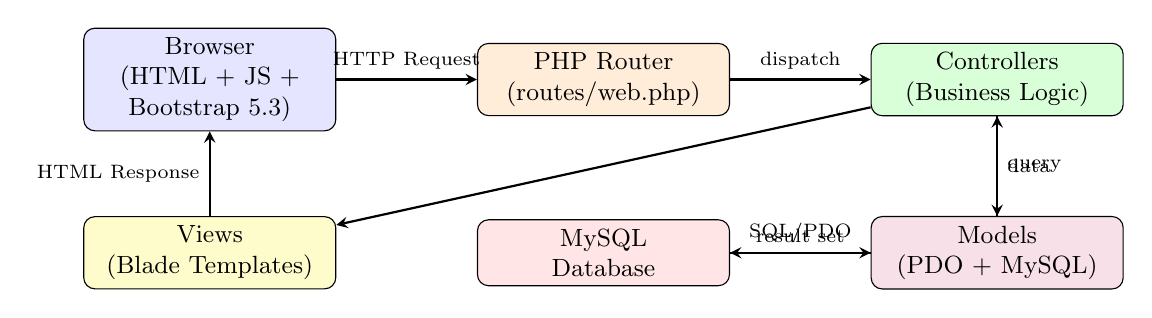
\begin{tikzpicture}[
    box/.style={draw, rounded corners=4pt, minimum width=3.2cm, minimum height=0.8cm, align=center, font=\small},
    arr/.style={->, thick, >=stealth},
    font=\small
]
% Browser
\node[box, fill=blue!10] (browser) at (0,0) {Browser\\(HTML + JS + \\Bootstrap 5.3)};
% Router
\node[box, fill=orange!15] (router) at (5,0) {PHP Router\\(routes/web.php)};
% Controllers
\node[box, fill=green!15] (ctrl) at (10,0) {Controllers\\(Business Logic)};
% Models / PDO
\node[box, fill=purple!12] (model) at (10,-2.2) {Models\\(PDO + MySQL)};
% DB
\node[box, fill=red!10] (db) at (5,-2.2) {MySQL\\Database};
% Views
\node[box, fill=yellow!20] (view) at (0,-2.2) {Views\\(Blade Templates)};

\draw[arr] (browser) -- node[above,font=\scriptsize]{HTTP Request} (router);
\draw[arr] (router) -- node[above,font=\scriptsize]{dispatch} (ctrl);
\draw[arr] (ctrl) -- node[right,font=\scriptsize]{query} (model);
\draw[arr] (model) -- node[above,font=\scriptsize]{SQL/PDO} (db);
\draw[arr] (db) -- node[above,font=\scriptsize]{result set} (model);
\draw[arr] (model) -- node[right,font=\scriptsize]{data} (ctrl);
\draw[arr] (ctrl) -- (view);
\draw[arr] (view) -- node[left,font=\scriptsize]{HTML Response} (browser);
\end{tikzpicture}
\end{center}

% ============================
% PAGE 8 — FOLDER STRUCTURE
% ============================
\newpage
\thispagestyle{plain}
{\large\bfseries Project Folder Structure}\\[0.6pt]
\rule{\textwidth}{0.6pt}

\vspace{0.4cm}

\begin{lstlisting}[language={},basicstyle=\ttfamily\small,frame=single,numbers=none]
project/
|-- app/
|   |-- Http/
|   |   |-- Controllers/
|   |   |   |-- Auth/          (Login, Register, OTP)
|   |   |   |-- Student/       (Dashboard, Booking, Search)
|   |   |   |-- Teacher/       (Profile, Availability, Sessions)
|   |   |   `-- Admin/         (Dashboard, Verification, Reports)
|   |   `-- Middleware/        (RoleMiddleware, AuthMiddleware)
|   |-- Models/
|   |   |-- User.php
|   |   |-- TeacherProfile.php
|   |   |-- StudentProfile.php
|   |   |-- Booking.php
|   |   |-- Message.php
|   |   `-- Review.php
|   `-- Services/              (BookingService, NotificationService)
|
|-- database/
|   `-- migrations/            (44 migration files)
|
|-- public/
|   |-- index.php              (Application entry point)
|   |-- images/                (Static images & SVGs)
|   `-- build/                 (Compiled CSS & JS assets)
|
|-- resources/
|   |-- views/
|   |   |-- landing.blade.php  (Public homepage)
|   |   |-- layouts/           (Shared layouts)
|   |   `-- pages/             (Student, Teacher, Admin pages)
|   |-- css/                   (Source stylesheets)
|   `-- js/                    (Source JavaScript)
|
|-- routes/
|   `-- web.php                (All application routes)
|
|-- .env                       (Environment config - DB, APP)
`-- composer.json              (PHP dependencies)
\end{lstlisting}

% ============================
% PAGE 9 — DATABASE TABLE STRUCTURE
% ============================
\newpage
\thispagestyle{plain}
{\large\bfseries Database Table Structure}\\[0.6pt]
\rule{\textwidth}{0.6pt}

\vspace{0.3cm}

% Table: users
\textbf{Table: users}\\[2pt]
\begin{tabular}{@{}L{3.2cm} L{3cm} L{7cm}@{}}
\toprule
\rowcolor{tableheader}\color{white}\textbf{Column} & \color{white}\textbf{Type} & \color{white}\textbf{Description} \\
\midrule
id & BIGINT (PK) & Auto-increment primary key \\
\rowcolor{tablealt}name & VARCHAR(255) & Full name of the user \\
email & VARCHAR(255) & Unique email (login identifier) \\
\rowcolor{tablealt}phone & VARCHAR(20) & Optional unique phone number \\
password & VARCHAR(255) & Bcrypt hashed password \\
\rowcolor{tablealt}role & ENUM & student / teacher / admin \\
status & ENUM & active / suspended / pending \\
\rowcolor{tablealt}avatar & VARCHAR & Profile picture path \\
email\_verified\_at & TIMESTAMP & Email verification timestamp \\
\rowcolor{tablealt}created\_at / updated\_at & TIMESTAMP & Record timestamps \\
\bottomrule
\end{tabular}

\vspace{0.4cm}

% Table: teacher_profiles
\textbf{Table: teacher\_profiles}\\[2pt]
\begin{tabular}{@{}L{3.2cm} L{3cm} L{7cm}@{}}
\toprule
\rowcolor{tableheader}\color{white}\textbf{Column} & \color{white}\textbf{Type} & \color{white}\textbf{Description} \\
\midrule
id & BIGINT (PK) & Primary key \\
\rowcolor{tablealt}user\_id & BIGINT (FK) & References users.id \\
bio & TEXT & Teacher biography \\
\rowcolor{tablealt}experience\_years & INT & Years of teaching experience \\
hourly\_rate & DECIMAL(8,2) & Per-session rate  \\
\rowcolor{tablealt}subjects & JSON & Array of subjects taught \\
languages & JSON & Spoken/teaching languages \\
\rowcolor{tablealt}rating\_avg & DECIMAL(3,2) & Aggregated review average \\
is\_verified & BOOLEAN & Admin-approved status \\
\bottomrule
\end{tabular}

\vspace{0.4cm}

% Table: bookings
\textbf{Table: bookings}\\[2pt]
\begin{tabular}{@{}L{3.2cm} L{3cm} L{7cm}@{}}
\toprule
\rowcolor{tableheader}\color{white}\textbf{Column} & \color{white}\textbf{Type} & \color{white}\textbf{Description} \\
\midrule
id & BIGINT (PK) & Primary key \\
\rowcolor{tablealt}student\_id & BIGINT (FK) & References users.id \\
teacher\_id & BIGINT (FK) & References users.id \\
\rowcolor{tablealt}slot\_id & BIGINT (FK) & References booking\_slots.id \\
start\_at / end\_at & DATETIME & Session time window \\
\rowcolor{tablealt}status & ENUM & pending/confirmed/completed \\
payment\_status & ENUM & unpaid/paid/refunded \\
\rowcolor{tablealt}price & DECIMAL(8,2) & Session price \\
subject & VARCHAR(100) & Subject for this session \\
\bottomrule
\end{tabular}

\vspace{0.4cm}

% Table: messages
\textbf{Table: messages}\\[2pt]
\begin{tabular}{@{}L{3.2cm} L{3cm} L{7cm}@{}}
\toprule
\rowcolor{tableheader}\color{white}\textbf{Column} & \color{white}\textbf{Type} & \color{white}\textbf{Description} \\
\midrule
id & BIGINT (PK) & Primary key \\
\rowcolor{tablealt}conversation\_id & BIGINT (FK) & Thread this message belongs to \\
sender\_id & BIGINT (FK) & References users.id \\
\rowcolor{tablealt}body & TEXT & Message content \\
read\_at & TIMESTAMP & Null until recipient reads \\
\rowcolor{tablealt}created\_at & TIMESTAMP & Sent timestamp \\
\bottomrule
\end{tabular}

% ============================
% PAGE 10 — LANDING PAGE SCREENSHOT
% ============================
\newpage
\thispagestyle{plain}
\begin{center}
    {\large\bfseries Landing Page}\\[4pt]
    \rule{\textwidth}{0.6pt}
    \vspace{0.3cm}

    \IfFileExists{landing.png}{
        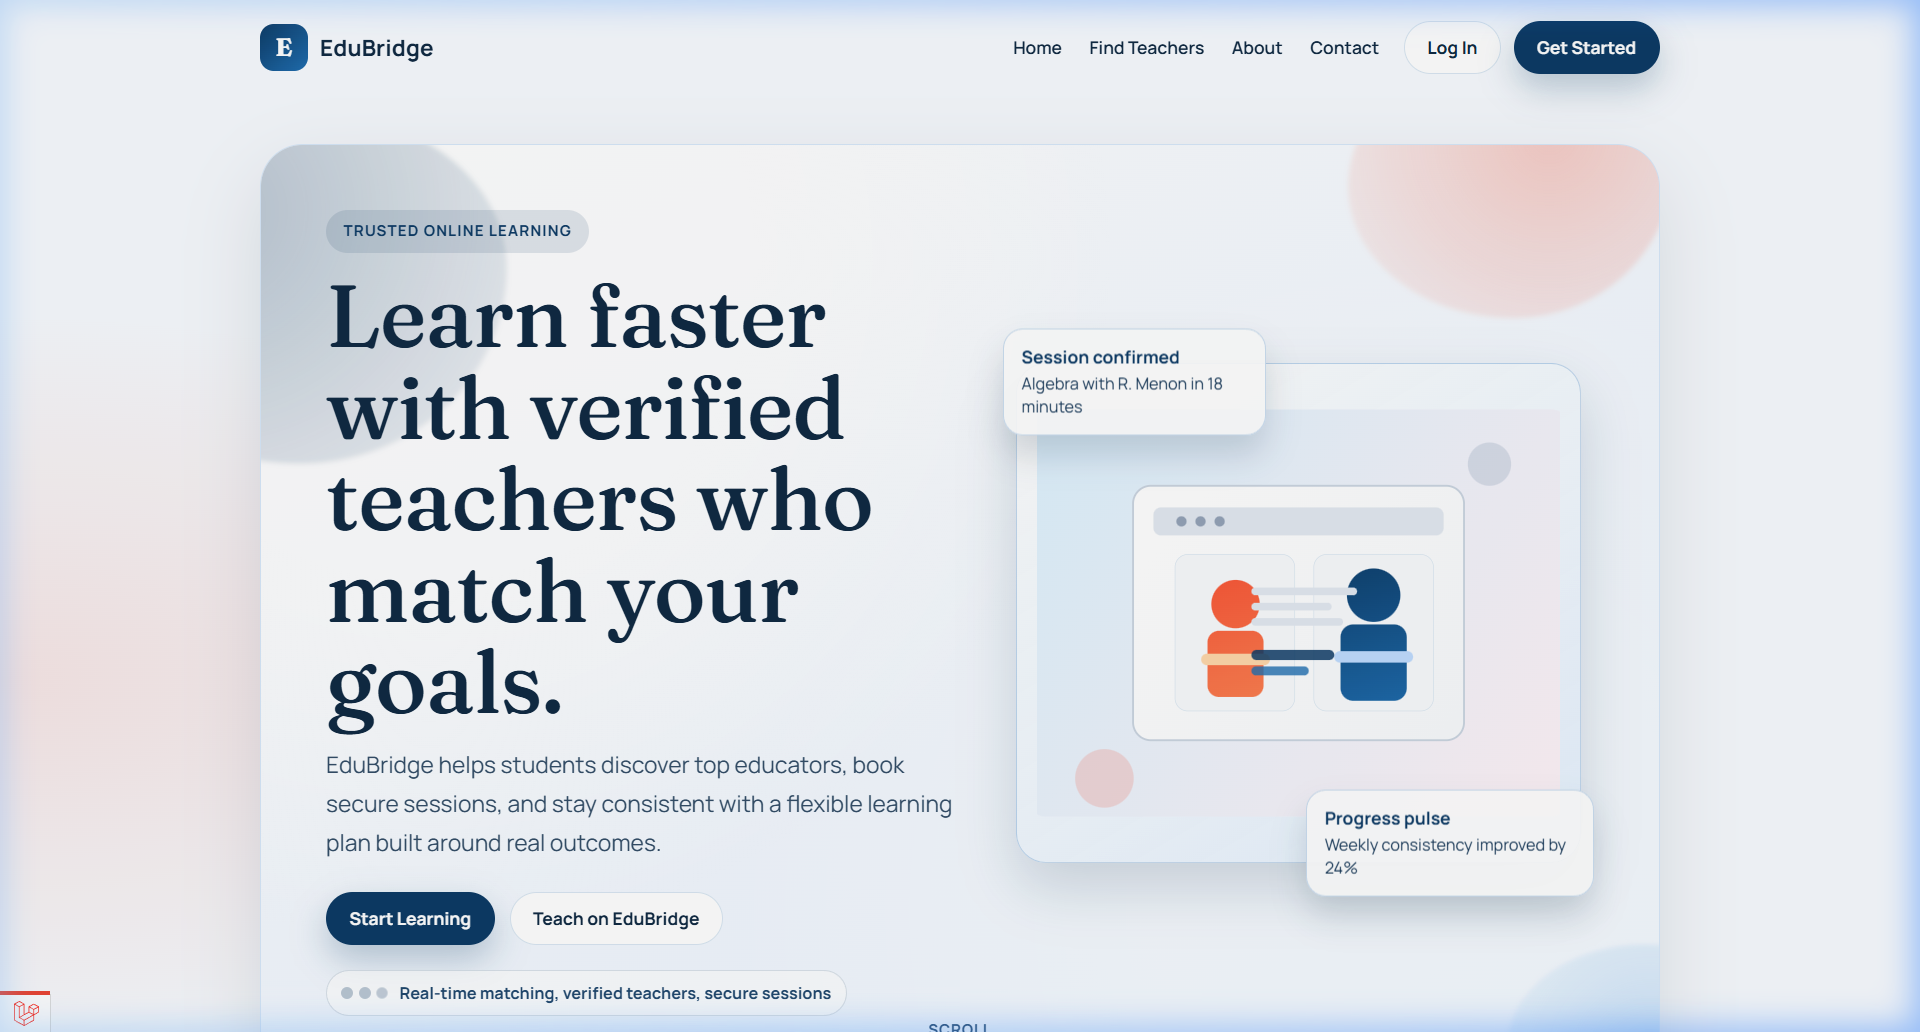
\includegraphics[width=\textwidth, height=0.88\textheight, keepaspectratio]{landing.png}
    }{[landing.png not found]}

    \vspace{0.3cm}
    \small\textit{Fig 1: EduBridge public homepage — hero section, stats, how-it-works, and CTA.}
\end{center}

% ============================
% PAGE 11 — STUDENT DASHBOARD
% ============================
\newpage
\thispagestyle{plain}
\begin{center}
    {\large\bfseries Student Dashboard}\\[4pt]
    \rule{\textwidth}{0.6pt}
    \vspace{0.3cm}

    \IfFileExists{student_dash.png}{
        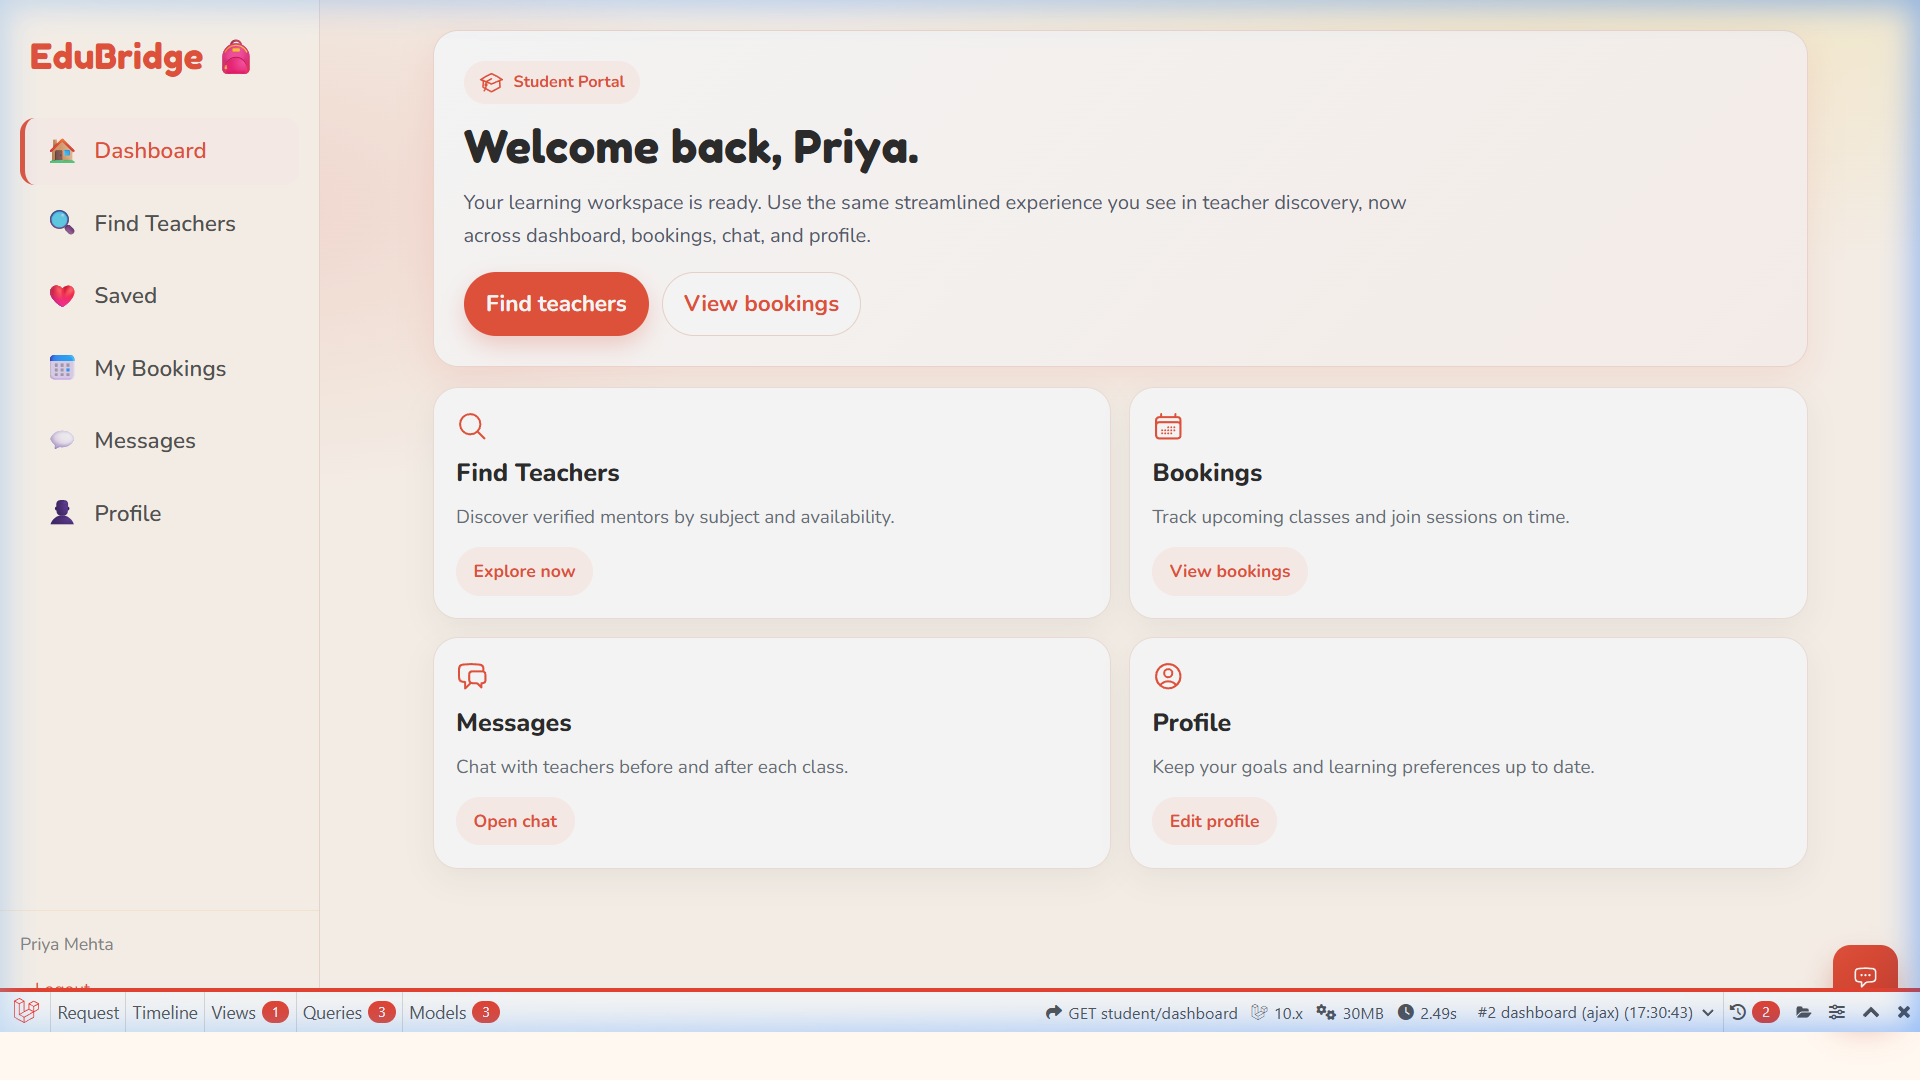
\includegraphics[width=\textwidth, height=0.88\textheight, keepaspectratio]{student_dash.png}
    }{[student\_dash.png not found]}

    \vspace{0.3cm}
    \small\textit{Fig 2: Student portal — upcoming sessions, quick search, and learning activity overview.}
\end{center}

% ============================
% PAGE 12 — TEACHER DASHBOARD
% ============================
\newpage
\thispagestyle{plain}
\begin{center}
    {\large\bfseries Teacher Dashboard}\\[4pt]
    \rule{\textwidth}{0.6pt}
    \vspace{0.3cm}

    \IfFileExists{teacher_dash.png}{
        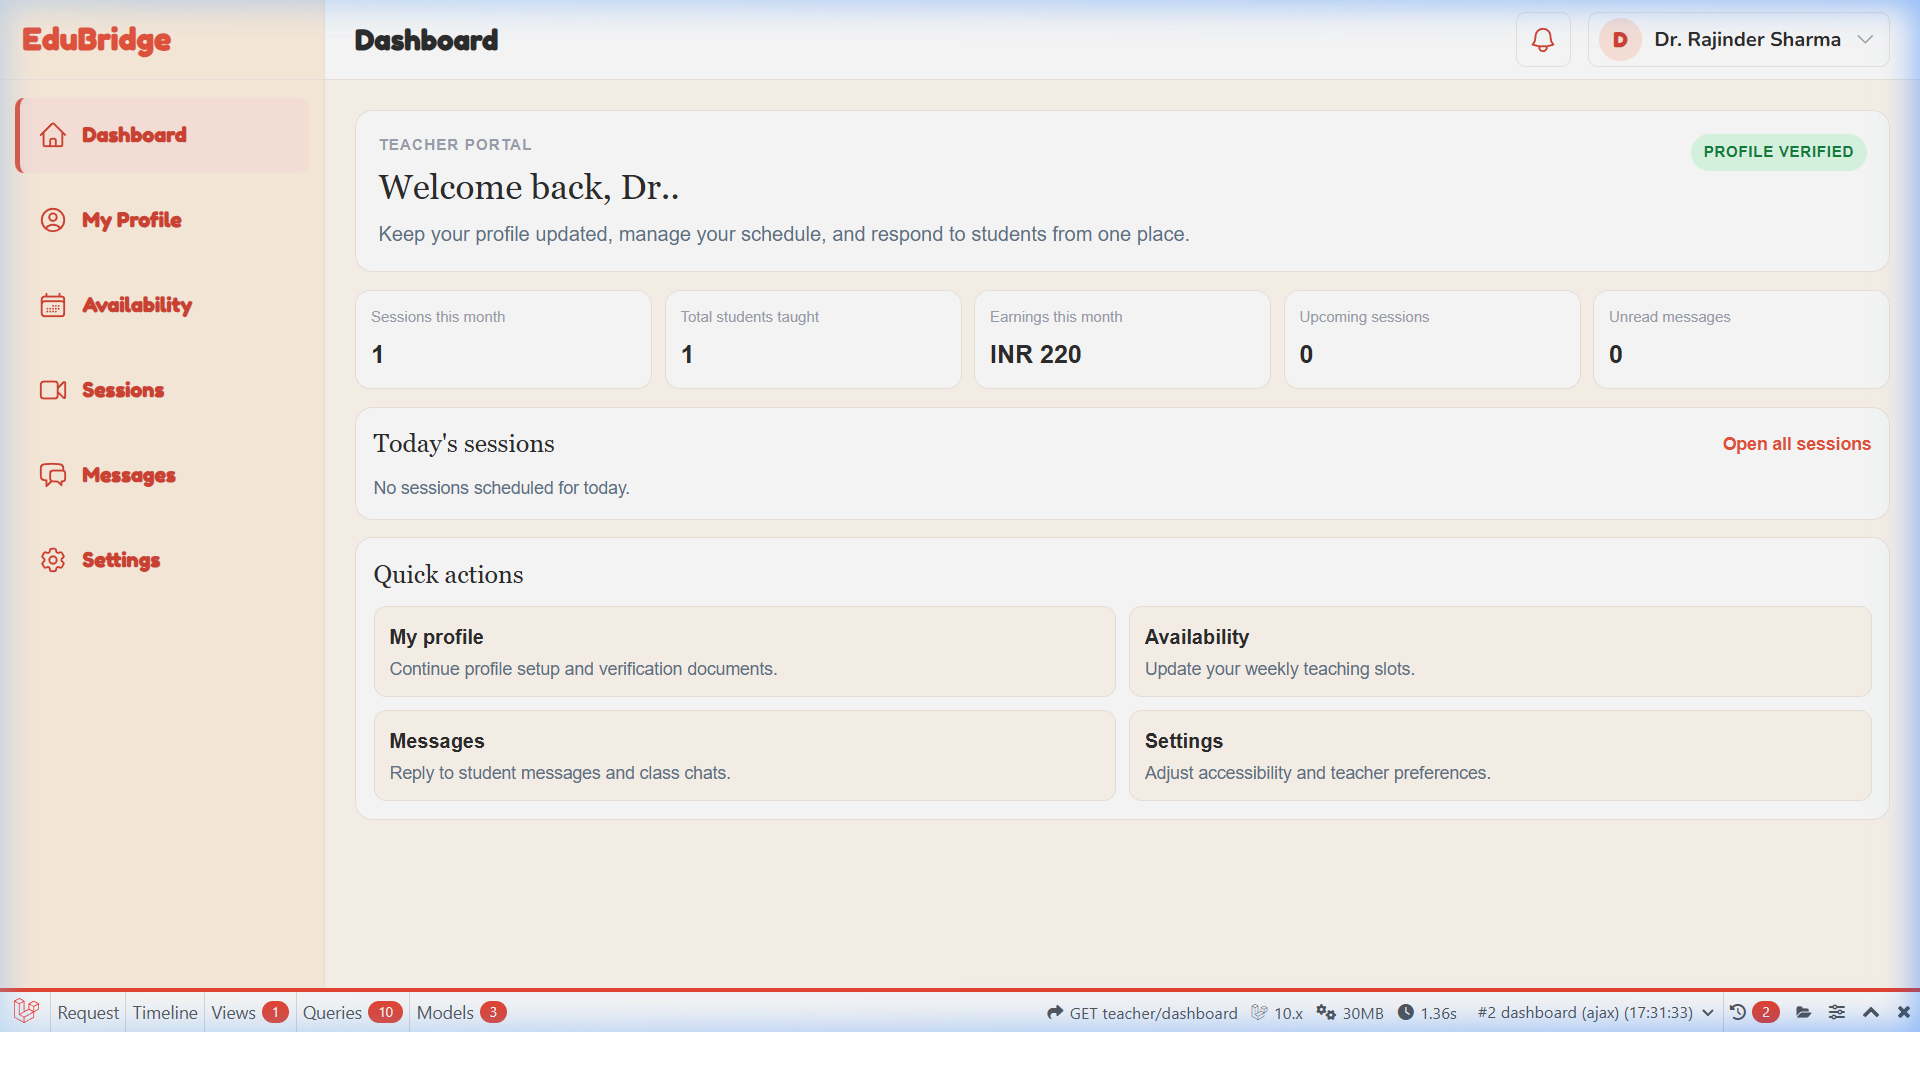
\includegraphics[width=\textwidth, height=0.88\textheight, keepaspectratio]{teacher_dash.png}
    }{[teacher\_dash.png not found]}

    \vspace{0.3cm}
    \small\textit{Fig 3: Teacher portal — booking forecasts, session management, and earnings overview.}
\end{center}

% ============================
% PAGE 13 — ADMIN DASHBOARD
% ============================
\newpage
\thispagestyle{plain}
\begin{center}
    {\large\bfseries Admin Dashboard}\\[4pt]
    \rule{\textwidth}{0.6pt}
    \vspace{0.3cm}

    \IfFileExists{admin_dash.png}{
        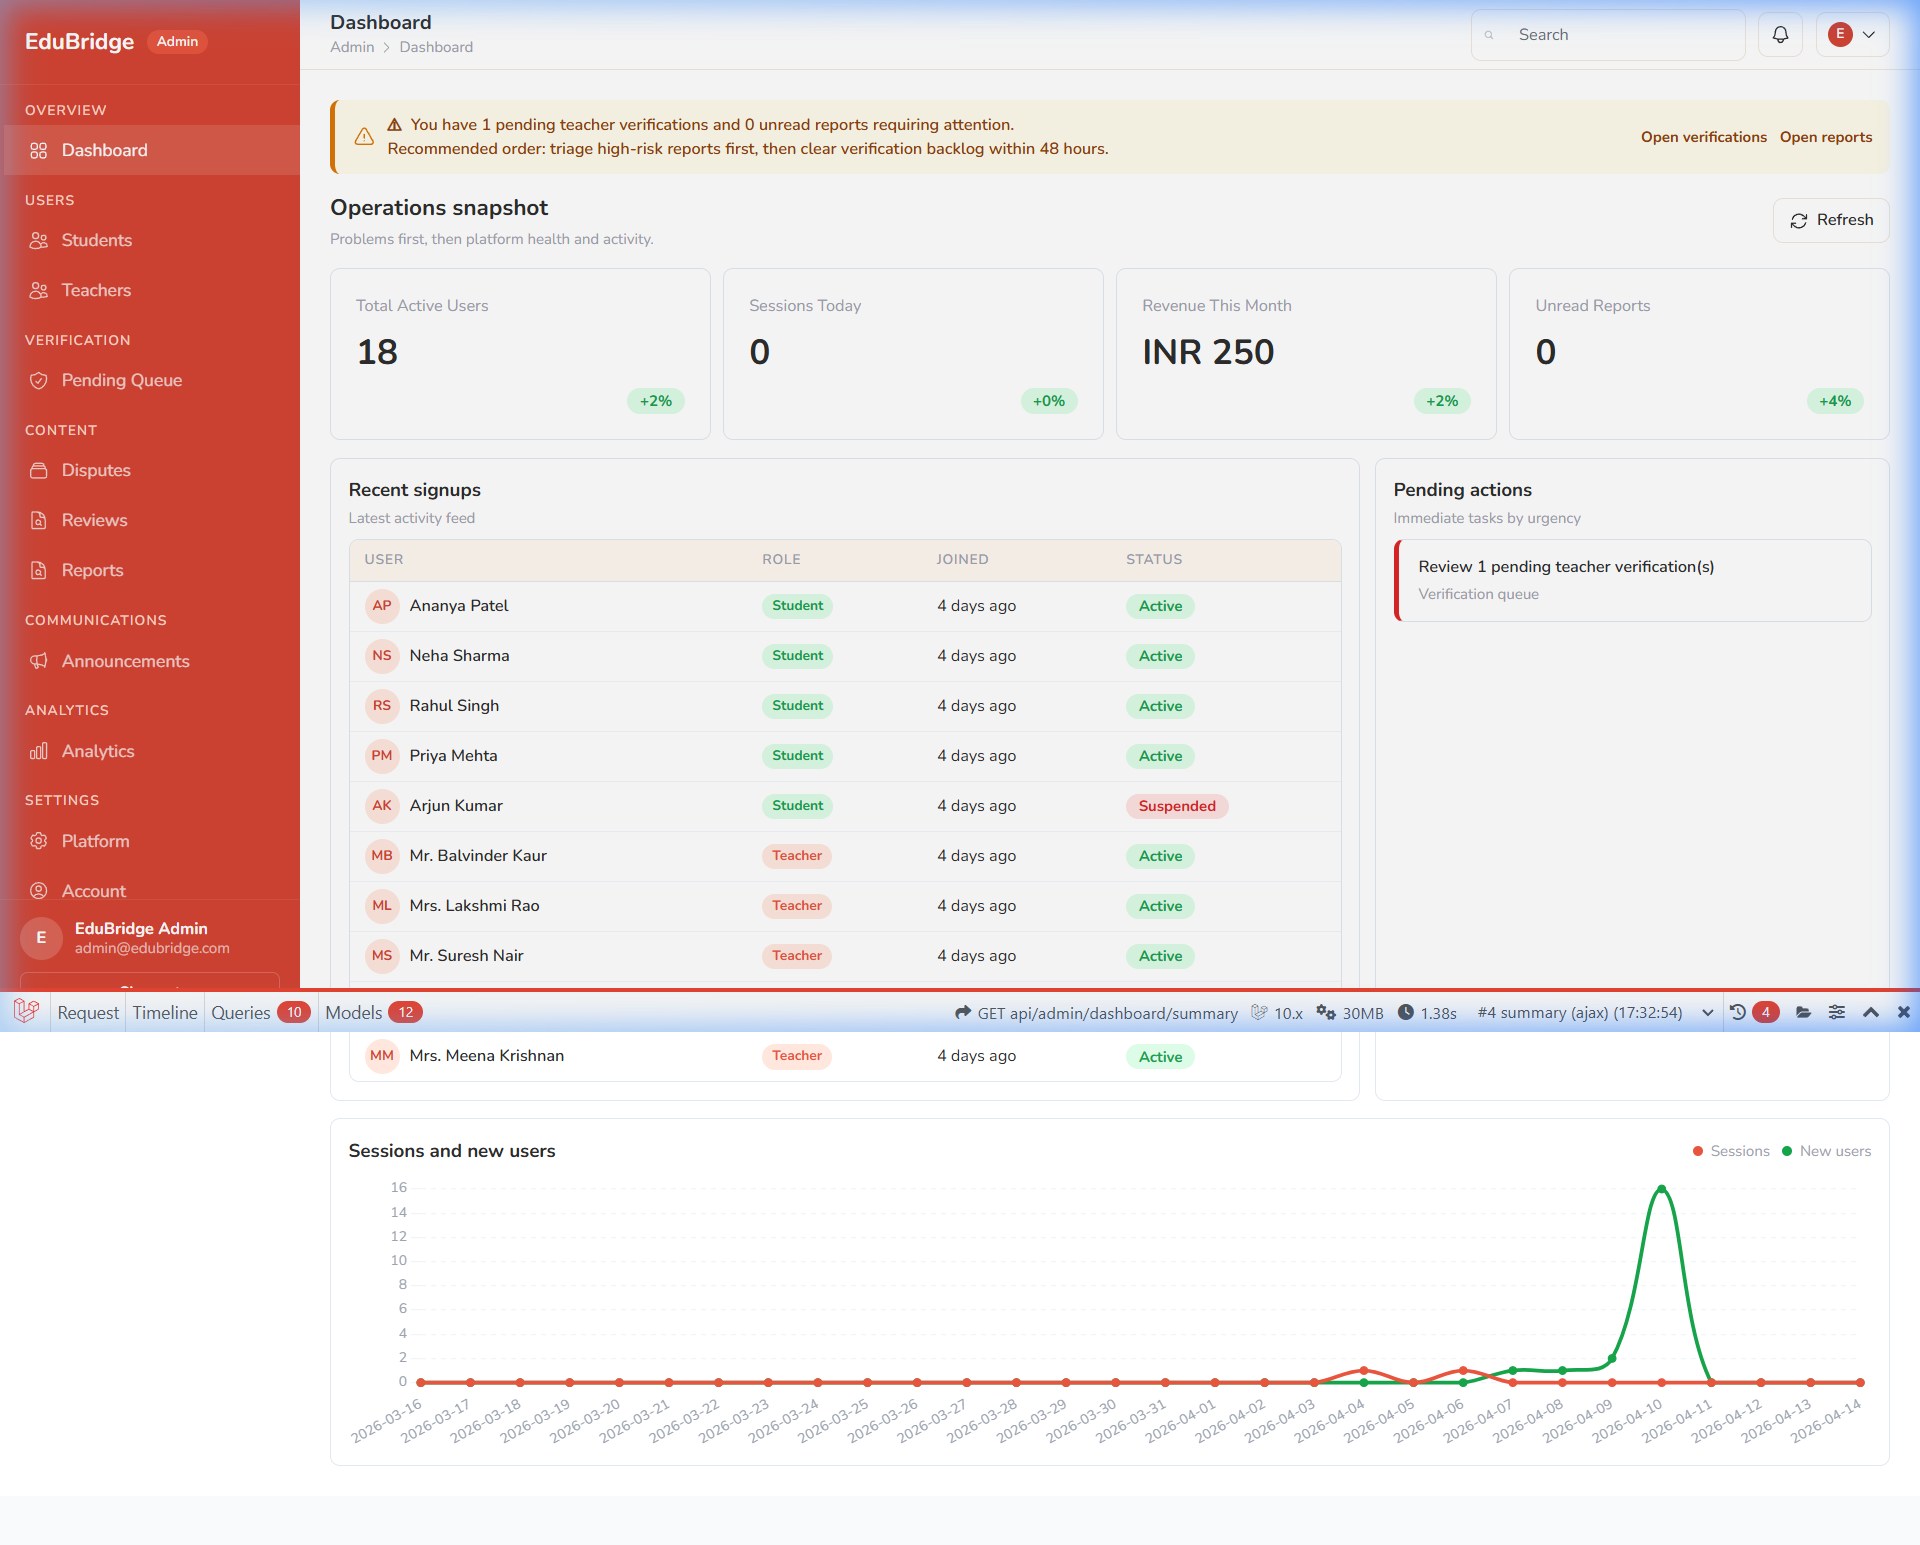
\includegraphics[width=\textwidth, height=0.88\textheight, keepaspectratio]{admin_dash.png}
    }{[admin\_dash.png not found]}

    \vspace{0.3cm}
    \small\textit{Fig 4: Admin panel — platform analytics, user management, and verification controls.}
\end{center}

% ============================
% PAGE 14 — WORKING SCREENSHOT 1
% ============================
\newpage
\thispagestyle{plain}
\begin{center}
    {\large\bfseries Application Working — Screen 1}\\[4pt]
    \rule{\textwidth}{0.6pt}
    \vspace{0.3cm}

    \IfFileExists{working1.png}{
        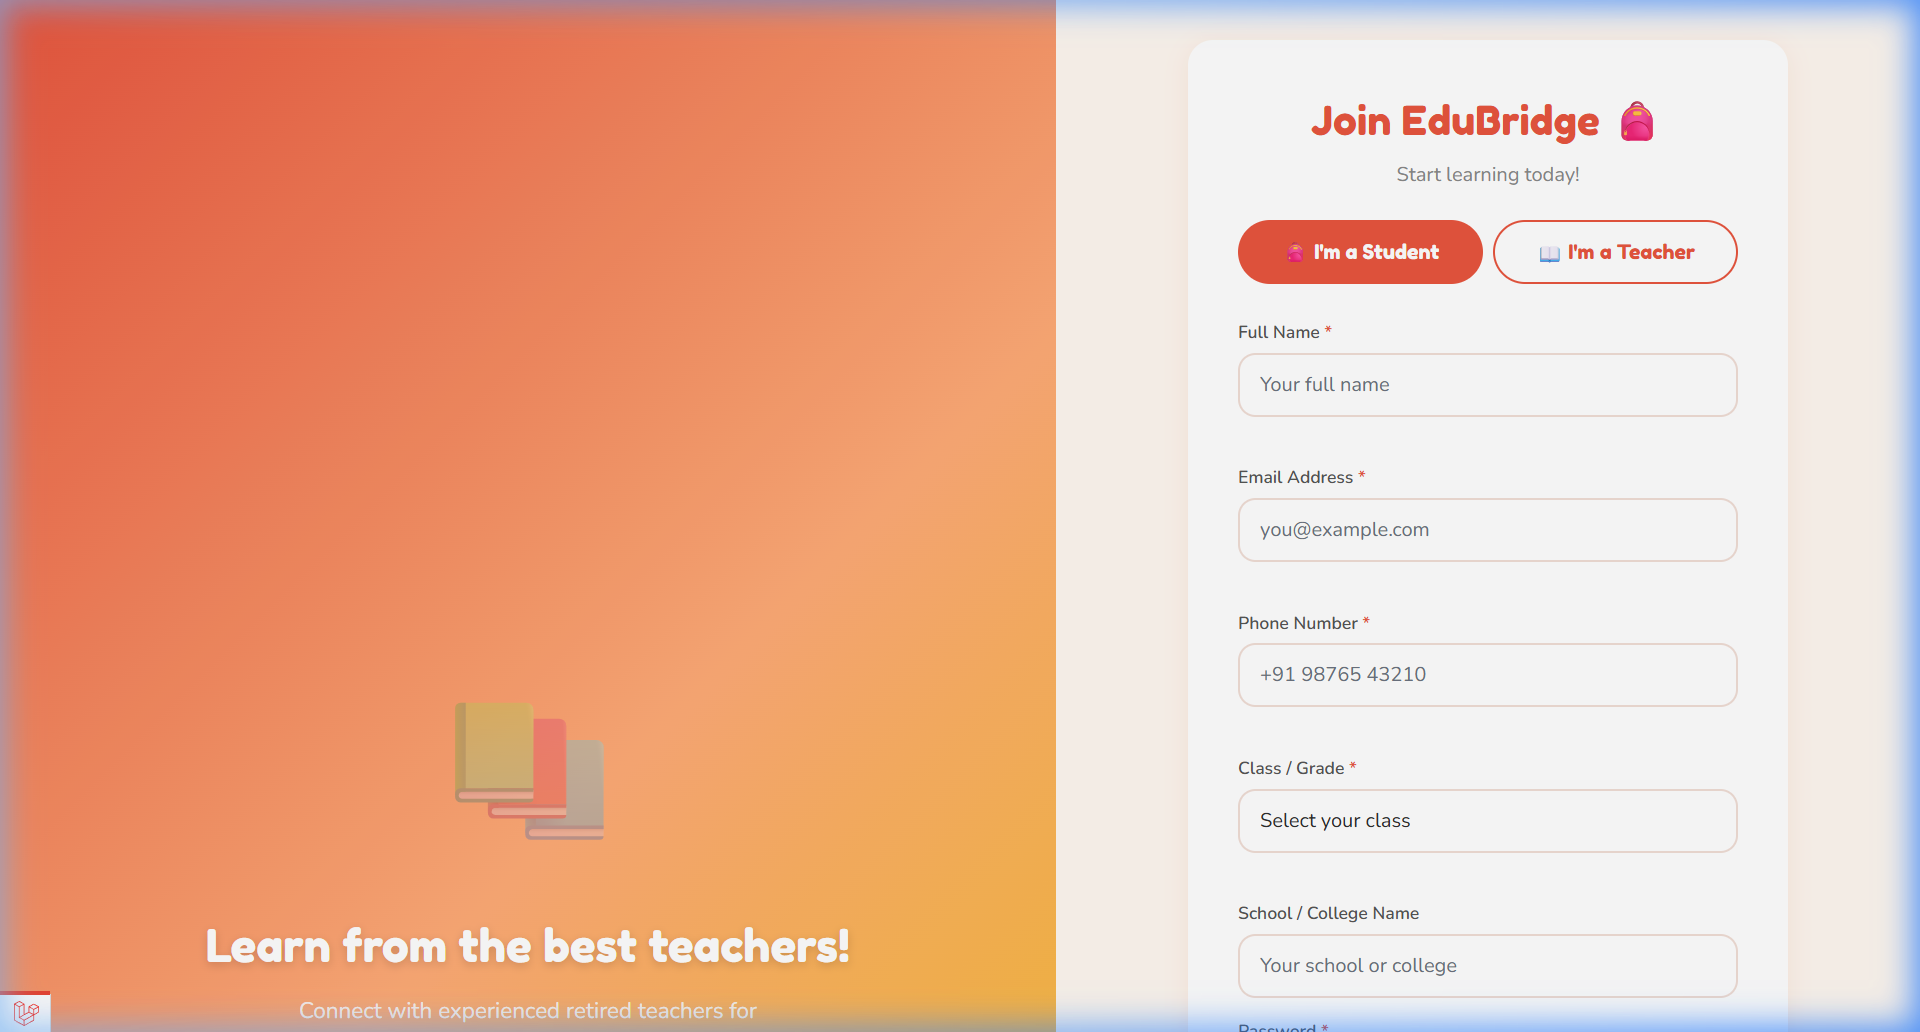
\includegraphics[width=\textwidth, height=0.88\textheight, keepaspectratio]{working1.png}
    }{[working1.png not found]}

    \vspace{0.3cm}
    \small\textit{Fig 5: Booking and session flow in action.}
\end{center}

% ============================
% PAGE 15 — WORKING SCREENSHOT 2
% ============================
\newpage
\thispagestyle{plain}
\begin{center}
    {\large\bfseries Application Working — Screen 2}\\[4pt]
    \rule{\textwidth}{0.6pt}
    \vspace{0.3cm}

    \IfFileExists{working2.png}{
        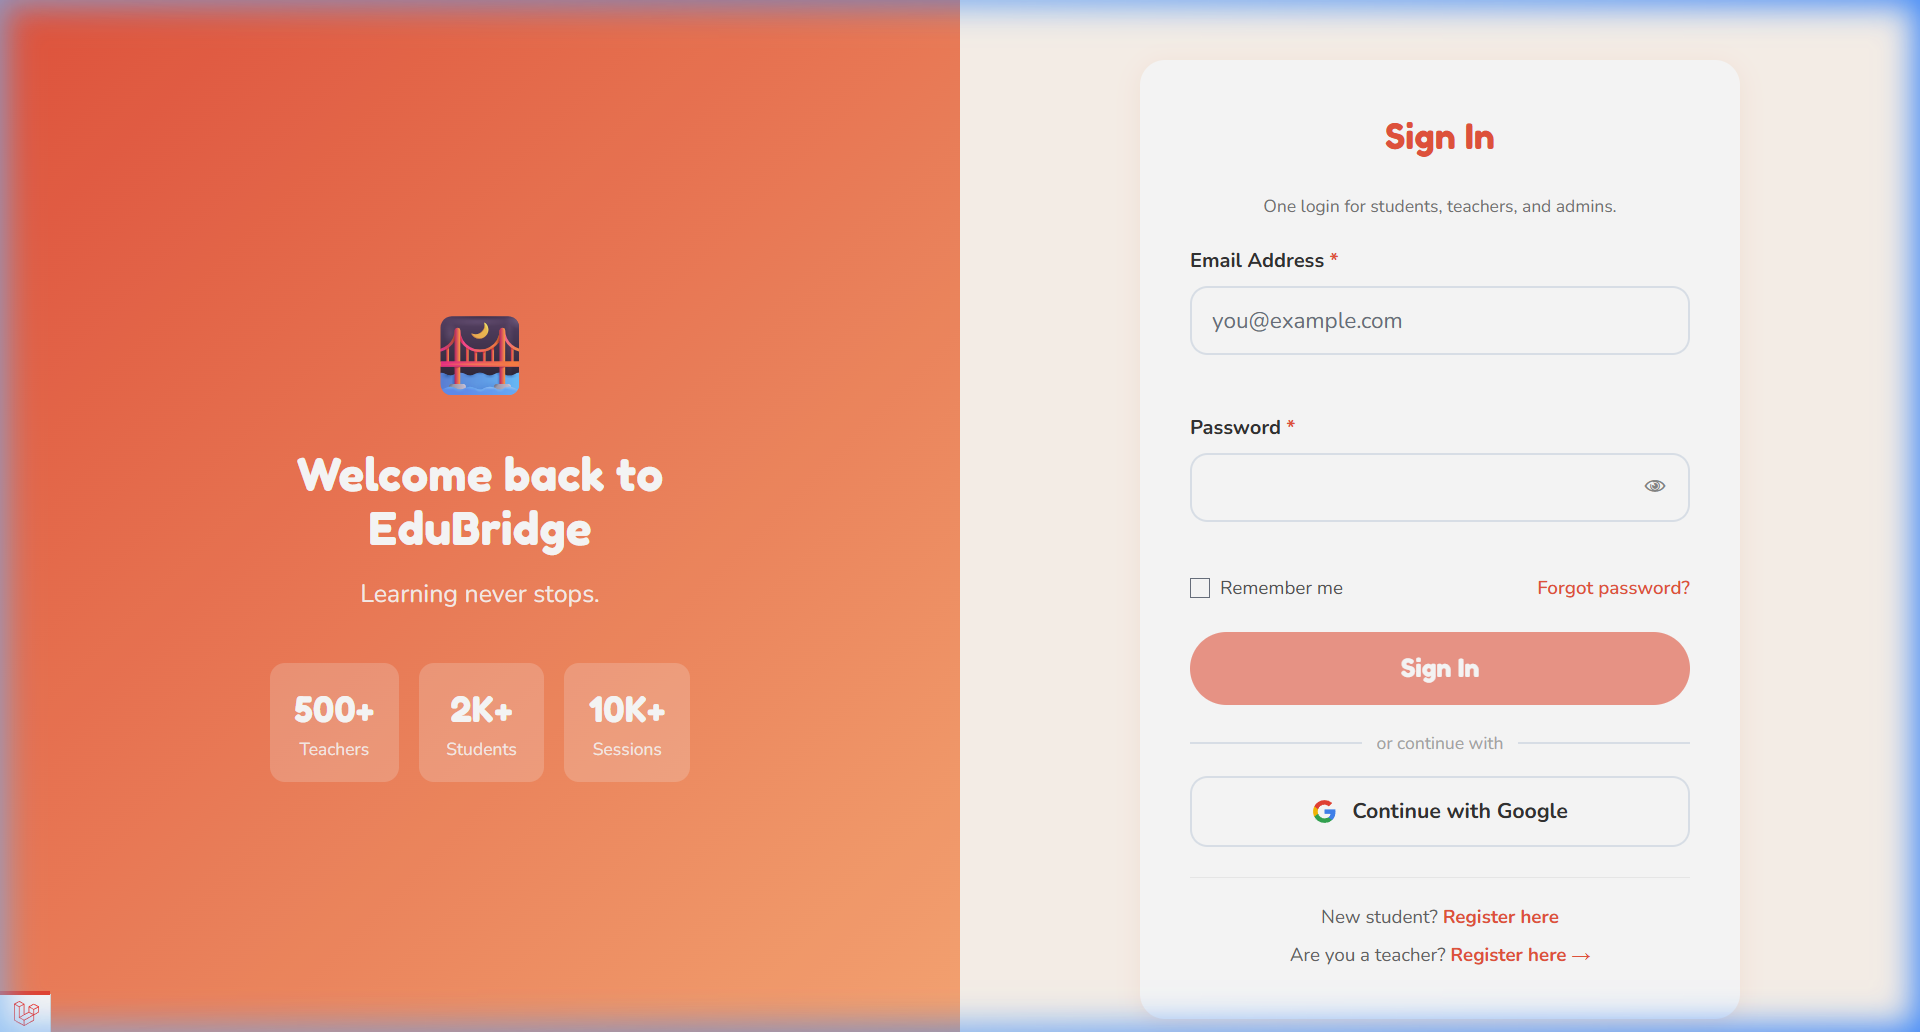
\includegraphics[width=\textwidth, height=0.88\textheight, keepaspectratio]{working2.png}
    }{[working2.png not found]}

    \vspace{0.3cm}
    \small\textit{Fig 6: Messaging and real-time communication interface.}
\end{center}

% ============================
% PAGE 16 — LANDING PAGE CODE
% ============================
\newpage
\thispagestyle{plain}
{\large\bfseries Landing Page Code (landing.blade.php)}\\[0.6pt]
\rule{\textwidth}{0.6pt}

\vspace{0.3cm}
\small Key structural HTML of the EduBridge public homepage (\texttt{resources/views/landing.blade.php}):

\begin{lstlisting}[language=html, caption={landing.blade.php -- Hero \& Stats Section}]
@extends('layouts.public')
@section('content')

<!-- ===== HERO SECTION ===== -->
<section class="hero-shell" id="landing-hero-shell">
    <div class="hero-backdrop" aria-hidden="true">
        <span class="blob blob-a"></span>
        <span class="blob blob-b"></span>
        <span class="blob blob-c"></span>
    </div>

    <div class="hero-grid">
        <div>
            <span class="hero-pill">Trusted online learning</span>
            <h1 class="hero-heading">
                Learn faster with verified teachers
                who match your goals.
            </h1>
            <p class="hero-subhead">
                EduBridge helps students discover top educators,
                book secure sessions, and stay consistent with a
                flexible learning plan built around real outcomes.
            </p>

            <div class="hero-actions">
                <a href="{{ route('student.register') }}"
                   class="btn-pill primary cta-shimmer"
                   id="landing-start-student">
                   Start Learning
                </a>
                <a href="{{ route('teacher.register') }}"
                   class="btn-pill secondary"
                   id="landing-start-teacher">
                   Teach on EduBridge
                </a>
            </div>

            <div class="hero-signal">
                Real-time matching, verified teachers, secure sessions
            </div>
        </div>

        <div class="hero-stage-shell">
            <div class="hero-stage" id="landing-hero-stage">
                <div class="hero-card top">
                    <strong>Session confirmed</strong>
                    Algebra with R. Menon in 18 minutes
                </div>
                <div class="hero-visual-frame">
                    <img src="{{ asset('images/hero-illustration.svg') }}"
                         alt="Student attending a live online class">
                </div>
                <div class="hero-card bottom">
                    <strong>Progress pulse</strong>
                    Weekly consistency improved by 24%
                </div>
            </div>
        </div>
    </div>
</section>

<!-- ===== STATS SECTION ===== -->
<section class="stats-section" id="landing-stats">
    <div class="stats-row">
        <article class="stat-card">
            <p class="stat-value"
               data-count="{{ $stats['teachers'] }}"
               data-suffix="+">0</p>
            <div>Active teachers</div>
        </article>
        <article class="stat-card">
            <p class="stat-value"
               data-count="{{ $stats['students'] }}"
               data-suffix="+">0</p>
            <div>Students enrolled</div>
        </article>
        <article class="stat-card">
            <p class="stat-value"
               data-count="{{ $stats['sessions'] }}"
               data-suffix="+">0</p>
            <div>Sessions completed</div>
        </article>
        <article class="stat-card">
            <p class="stat-value"
               data-count="{{ $stats['reviews'] }}"
               data-suffix="+">0</p>
            <div>Verified reviews</div>
        </article>
    </div>
</section>

<!-- ===== HOW IT WORKS ===== -->
<section class="section-shell">
    <h2 class="section-title">
        A smooth loop from discovery to measurable progress.
    </h2>
    <div class="steps-grid">
        <article class="step-card">
            <span class="step-index"><strong>1</strong></span>
            <h3>Explore teachers</h3>
            <p>Search by subject, ratings, and teaching style.</p>
        </article>
        <article class="step-card">
            <span class="step-index"><strong>2</strong></span>
            <h3>Book instantly</h3>
            <p>Pick open time slots and confirm in one flow.</p>
        </article>
        <article class="step-card">
            <span class="step-index"><strong>3</strong></span>
            <h3>Attend live class</h3>
            <p>Join interactive sessions with structured content.</p>
        </article>
        <article class="step-card">
            <span class="step-index"><strong>4</strong></span>
            <h3>Review outcomes</h3>
            <p>Leave feedback and tune your learning trajectory.</p>
        </article>
    </div>
</section>

@endsection
\end{lstlisting}

% ============================
% PAGE 17 — TESTING AND RESULTS
% ============================
\newpage
\thispagestyle{plain}
{\large\bfseries Testing \& Results}\\[0.6pt]
\rule{\textwidth}{0.6pt}

\vspace{0.4cm}
\textbf{Testing Approach}

\begin{itemize}[leftmargin=1.5em, itemsep=2pt]
    \item \textbf{Functional Testing} — Each module (registration, login, booking, messaging) tested manually against expected behaviour.
    \item \textbf{Role-Based Access Testing} — Verified that Student, Teacher, and Admin routes are protected and inaccessible across roles.
    \item \textbf{Validation Testing} — All form inputs tested with invalid data to confirm proper error feedback.
    \item \textbf{Database Integrity} — Foreign key constraints, cascade deletes, and PDO prepared statements verified.
\end{itemize}

\vspace{0.5cm}
\textbf{Sample Test Results}

\vspace{0.2cm}
\begin{tabular}{@{}C{0.5cm} L{4.8cm} L{4cm} L{2.5cm} C{1.5cm}@{}}
\toprule
\rowcolor{tableheader}\color{white}\textbf{\#} & \color{white}\textbf{Test Case} & \color{white}\textbf{Input} & \color{white}\textbf{Expected} & \color{white}\textbf{Result} \\
\midrule
1 & Student registers with valid data & Name, email, password & Account created, redirect to dashboard & \textcolor{green!60!black}{Pass} \\
\rowcolor{tablealt}2 & Login with wrong password & Wrong password & ``Invalid credentials'' error & \textcolor{green!60!black}{Pass} \\
3 & Student books an available slot & Select slot + confirm & Booking saved, status = pending & \textcolor{green!60!black}{Pass} \\
\rowcolor{tablealt}4 & Teacher accesses admin dashboard & Admin URL & Redirected to teacher dashboard & \textcolor{green!60!black}{Pass} \\
5 & Send message in conversation & Message text & Stored and displayed instantly & \textcolor{green!60!black}{Pass} \\
\rowcolor{tablealt}6 & Admin verifies a teacher & Approve action & Teacher status set to verified & \textcolor{green!60!black}{Pass} \\
7 & SQL injection attempt on login & \texttt{' OR 1=1 --} & Query blocked by PDO & \textcolor{green!60!black}{Pass} \\
\rowcolor{tablealt}8 & Empty form submission & No input & Validation errors displayed & \textcolor{green!60!black}{Pass} \\
9 & Student leaves a review & Rating + comment & Saved, rating average updated & \textcolor{green!60!black}{Pass} \\
\rowcolor{tablealt}10 & Responsive layout on mobile & 375px viewport & Layout adjusts via Bootstrap grid & \textcolor{green!60!black}{Pass} \\
\bottomrule
\end{tabular}

\vspace{0.5cm}
\textbf{Summary:} All 10 test cases passed. No critical bugs were found during testing. The application handles invalid inputs, unauthorised access, and SQL injection attempts correctly.

% ============================
% PAGE 18 — CONCLUSION + FUTURE SCOPE
% ============================
\newpage
\thispagestyle{plain}
{\large\bfseries Conclusion \& Future Scope}\\[0.6pt]
\rule{\textwidth}{0.6pt}

\vspace{0.4cm}
\textbf{Conclusion}

\vspace{0.2cm}
EduBridge successfully demonstrates a complete, functional web application for online tutoring management. The project covers the full development lifecycle — from database design and server-side PHP logic to a responsive, user-friendly front-end using Bootstrap 5.3.

\vspace{0.3cm}
The three-portal architecture (Student, Teacher, Admin) ensures clean separation of concerns and role-appropriate interfaces. PDO prepared statements and bcrypt hashing enforce security. The booking, messaging, and review systems work cohesively to deliver a practical edu-tech product.

\vspace{0.3cm}
The project achieves all stated objectives and provides a solid foundation for a scalable real-world educational platform.

\vspace{0.6cm}
\textbf{Future Scope}

\begin{itemize}[leftmargin=1.5em, itemsep=4pt]
    \item \textbf{Payment Gateway Integration} — Connect Razorpay or Stripe for live payment processing and automated teacher payouts.
    \item \textbf{Video Conferencing} — Embed WebRTC or Jitsi for in-platform video sessions, eliminating the need for external tools.
    \item \textbf{PWA / Mobile App} — Convert the platform into a Progressive Web App or build a native mobile client (Flutter/React Native).
    \item \textbf{AI Teacher Matching} — Implement an ML-based recommendation engine that suggests teachers based on the student's learning history and preferences.
    \item \textbf{Email \& SMS Notifications} — Automated reminders for upcoming sessions, booking confirmations, and review requests.
    \item \textbf{Group Live Classes} — Expand the platform to support multi-student paid group sessions with shared whiteboards.
    \item \textbf{Cloud Deployment} — Migrate from XAMPP to a cloud server (AWS / DigitalOcean) with HTTPS, CI/CD pipelines, and automated backups.
\end{itemize}

% ============================================================
\end{document}
